\chapter{Design} \label{chapter:design}

\section{Overview}

The project can be split into two main sections: the front-end mobile application that the user can interact with and the back-end server to store data and communicate with the mobile app.

These two sections link together very closely and are both required to produce a working implementation. It is therefore extremely important to not only consider the design of the user interface but also more technical aspects, such as the way the user's data is stored in the database and how the API will communicate with the mobile app.

\section{Project Requirements} \label{section:requirements}

Based on the broad objectives from Section \ref{section:objectives} and the background research conducted in Chapter \ref{chapter:background}, a detailed list of technical requirements was created. These requirements essentially map to features that need to be designed and implemented in the project. The objective that each requirement supports is shown in brackets.

% add paragraph here or after requirements as to why you chose to do each one

\begin{enumerate}[label=\textbf{Req \arabic*}]
    \item Build a fully functioning iOS application with a simple design and an easy-to-use user interface (\textbf{Obj 3}).
    \item Allow the user to track the routes of the walks they go on, as well as provide statistics about the walk such as distance travelled and number of steps (\textbf{Obj 1}).
    \item During a walk, the application should display certain points of interest on a map near the user's current location (\textbf{Obj 2}).
    \item Each user should be able to register an account within the application and publish their tracked walks to their profile (\textbf{Obj 1}).
    \item Users should be able to invite other users to go on a walk together and schedule this walk for a point in the future (\textbf{Obj 1}).
    \item The application should contain gamification - each user will have a score on their profile based on how far they have walked in total, how many walks they have been on and how often they go for a walk (\textbf{Obj 1}).
\end{enumerate}

With these requirements established, I was able to begin the design process for both the front and back-end in accordance with the features described.

\section{Mobile App Design}

% design of app
% how screens are organised
% survey

The mobile application produced for this project is the front-end product that the user interacts with. It therefore needs to have a sleek user interface and be well organised and easy to use.

\subsection{User Interface} \label{subsection:user-interface}

Before any implementation took place, I conducted an initial survey to find out various technical details such as which features would be most popular, which in turn allowed me to generate some design mockups of the application.

I chose to try and follow the iOS Human Interface Guidelines \cite{AppleInc.c} provided by Apple. These guidelines cover the basic design principles that should be used when creating a clear, fluid and easy to use iOS application. The guidelines provided a number of concepts to help structure how data is organised within the app.

Different app-level sections of an iOS application should be split using the tab bar UI element. This is a bar that is constantly present at the bottom of the screen containing a number of icons that the user can select to switch between sections of the app. The app for this project can be split into three main sections: tracking walks, managing sent and received walk invites and viewing the user's profile. From this, I was able to construct mockups for each of these sections -- shown in Figure \ref{fig:initial-mockups}.

\begin{figure}[hbt]
  \centering
  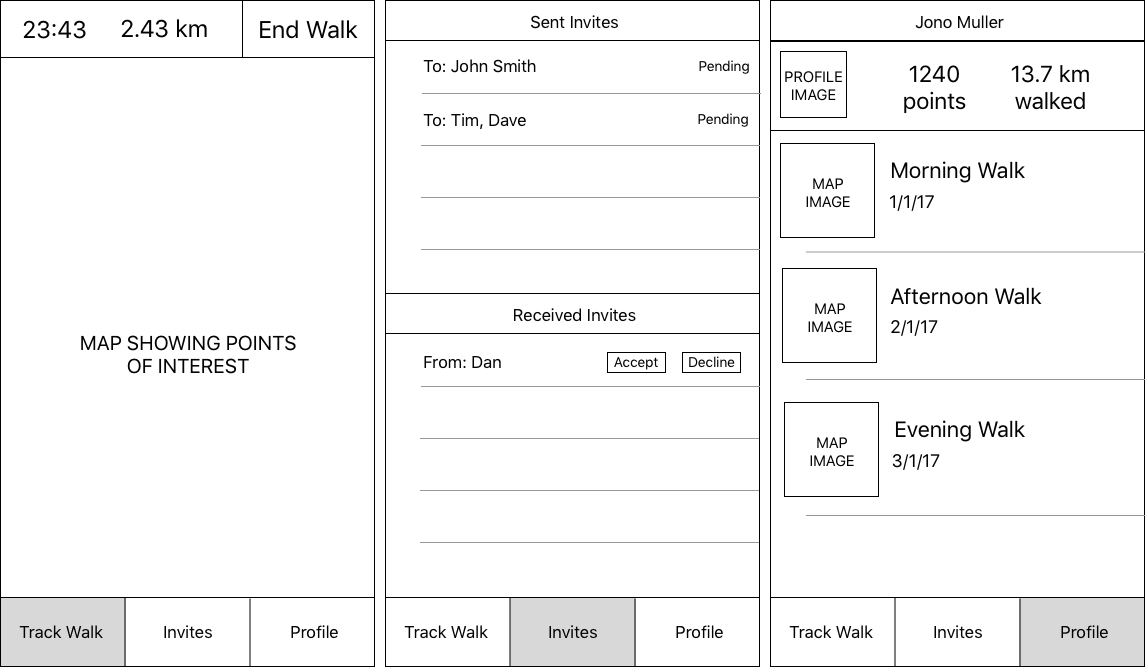
\includegraphics[width=\textwidth]{initial-mockups}
  \caption{Initial mockups of the mobile application, showing how the app is split up into three main sections using the tab bar design.}
  \label{fig:initial-mockups}
\end{figure}

As the design process wore on, I was able to create more detailed mockups utilising more of the resources from the Human Interface Guidelines. I updated the mockups so that each screen of the application contained a navigation bar -- a widely-used UI design pattern in iOS. Setting this as a standard throughout the app provides the user with a constant place where they can navigate between screens of the app and alter content that is displayed on the current screen. I also chose to use collections to display the list of walks on a user's profile instead of the standard tabular method, mainly due to its more visual approach. The updated mockups for the profile view containing collections and the walk detail view showing a navigation bar can be seen in Figure \ref{fig:profile-detail-mockup}.

\begin{figure}[hbt]
  \centering
  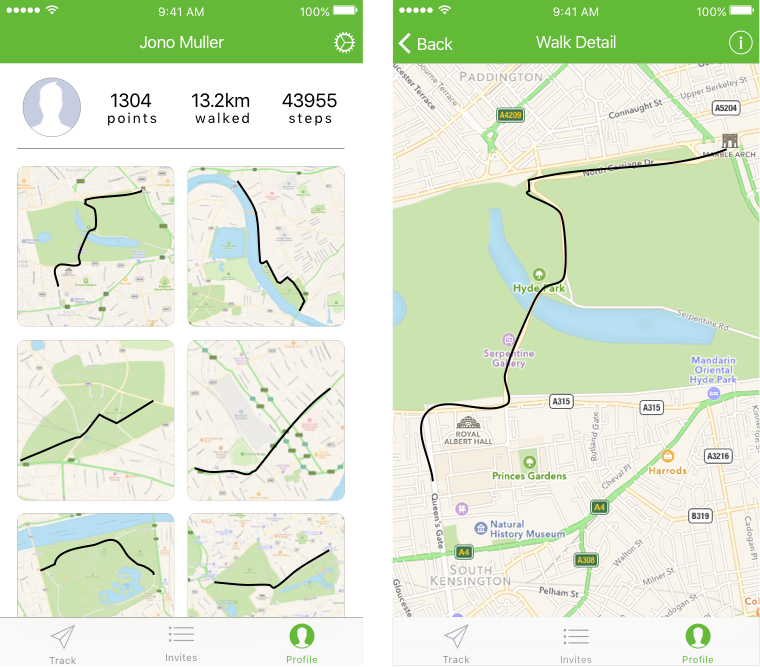
\includegraphics[width=0.9\textwidth]{profile-detail-mockup}
  \caption{Updated mockups of the user profile view (left) that contains a collection of the user's walks, and the walk detail view (right) that is presented when one of the walks from the profile view is selected.}
  \label{fig:profile-detail-mockup}
\end{figure}

Another design element that I chose to use is a segmented control -- a switch containing two or more elements to toggle between different views, normally used to switch between similar content in the same section. Its purpose fits nicely into the invites section of the app, where both sent and received invites need to be displayed but each contains similar information. By using a segmented control, placed in the navigation bar to maximise screen content, users will be able to toggle between viewing their sent and received invites from within the invites tab. The full mockup is displayed in Figure \ref{fig:invites-mockup}.

\begin{figure}[hbt]
  \centering
  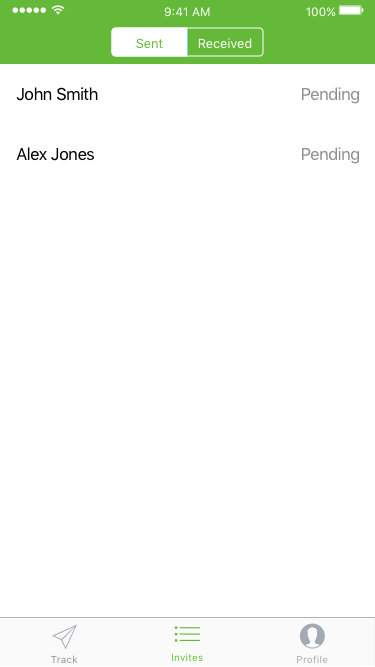
\includegraphics[width=0.45\textwidth]{invites-mockup}
  \caption{Redesigned mockup of the invites section of the application, using a segmented control in the navigation bar to switch between viewing sent and received invites.}
  \label{fig:invites-mockup}
\end{figure}

% login, register mockups
% updated track walk mockups
% summary

\subsection{Model-View-Controller Design Pattern}

An encouraged design pattern to use when creating a mobile application, namely an iOS app, is the Model-View-Controller (MVC) pattern. When following this pattern, objects in an application are split into three layers. Relating to this project, the three layers will be used as follows:

\begin{itemize}
  \item \textbf{Model} stores the data within the application and specifies the logic that alters that data. For this project the model will contain data relating to user information, tracked walk details and invites.
  
  \item \textbf{View} specifies objects that are visible to the user. They can either be used directly from Apple's UIKit framework or customised and reused as needed. The main view objects that are used for this project include \texttt{MKMapView} that displays a map on screen and \texttt{UITableView}, useful for displaying an indefinite list of data such as a list of invites.
  
  \item \textbf{Controller} is a medium between the other two layers. It deals with updating the \textbf{Model} based on changes from the \textbf{View} and vice versa. The UIKit framework provides default classes to handle this layer, such as a \texttt{UITableViewController} class that updates a \texttt{UITableView}. A diagram showing how the three layers link together in the project can be seen in Figure \ref{fig:mvc-diagram}.
\end{itemize}

\begin{figure}[hbt]
  \centering
  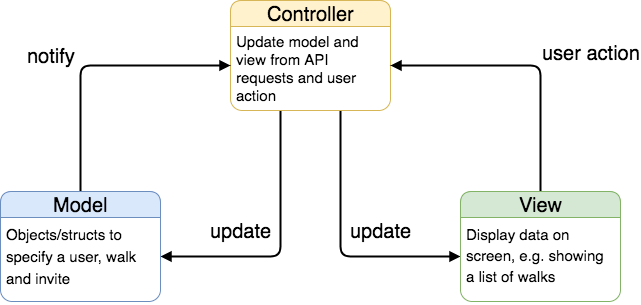
\includegraphics[width=0.8\textwidth]{mvc-diagram}
  \caption{How the Model-View-Controller design pattern links together for this application.}
  \label{fig:mvc-diagram}
\end{figure}


% mvc
% tab-bar
% human interface guidelines

\section{API Design}

% REST model, specific endpoints, etc.

Given that the API dealt primarily with JSON because of its easy connectivity with Node.js and MongoDB, responses were returned in JSON. Each response contained a success boolean as one of the values in JSON, determining whether the request was successful or not. HTTP error codes were used to determine the nature of a response as well, but the success flag was useful for error checking within the API.

The following section discusses how the structure of the API is organised as well as how the data was split up in the database.

% add image of how api links to app?

\subsection{Database Models}

% types of models – user, walk, invite, etc.

The data that needed to be stored in the database was split into multiple tables, or collections as they are called in MongoDB, to organise the data effectively. The full UML diagram showing each table's fields and how they link together can be seen in Figure \ref{fig:db-models}. A description of each of the four main tables is as follows:

\begin{itemize}
  \item \textbf{User} stores information about a user, created when they register. It contains cumulative values for the user's score, how far they have walked and how many steps they have taken. It also stores a user's device token, which is used to send a notification to a user's phone when inviting someone to go on a walk.

  \item \textbf{Invite} contains details of an invite sent from one user to one or more other users. Each user in the list of invite recipients contains a boolean flag to indicate whether that user has accepted the invite.

  \item \textbf{Achievement} is a fairly basic collection that stores the type of achievement that was gained from tracking a walk as well as how many points were gained from that achievement. The gamification and achievement aspect of the project is discussed in more detail in Section \ref{subsection:implementation-gamification}.
 
  \item \textbf{Walk} stores the details and representation of a walk, given a list of coordinates. It contains a reference to which user(s) tracked the walk, along with what achievements were gained.
\end{itemize}

% add required fields
% write description about each one?

\begin{figure}[hbt]
  \centering
  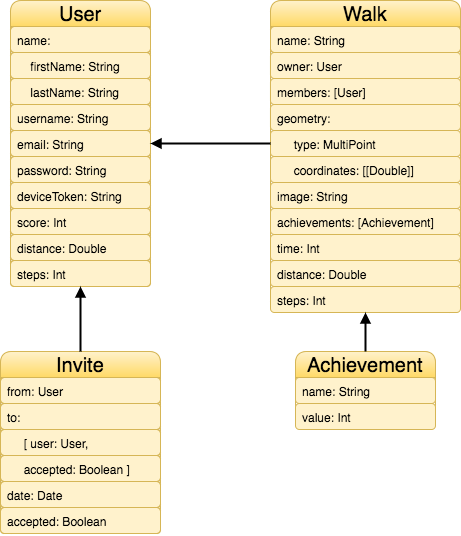
\includegraphics[width=0.7\textwidth]{db-models}
  \caption{Diagram of the different database models used in the project. Arrows indicate where a field in a table references another table.}
  \label{fig:db-models}
\end{figure}

\subsection{Endpoint Structure}

The REST architectural style dictates that each element in the web service uniquely identifies one resource. Based on this, I chose to create a number of endpoints that each provided access to a resource on the server. An endpoint is a reference to a uniform resource indicator (URI) that exposes a resource on the server, given a specific HTTP method. These endpoints were grouped into similar categories, where each category is known as a route, to provide clarity to the client. For example, all endpoints that update user information are grouped under the \texttt{/users/} route, with specific user endpoints a subpath of this route. The diagram representation of all of the routes used for the API is shown in Figure \ref{fig:api-routes}.

\begin{figure}[hbt]
  \centering
  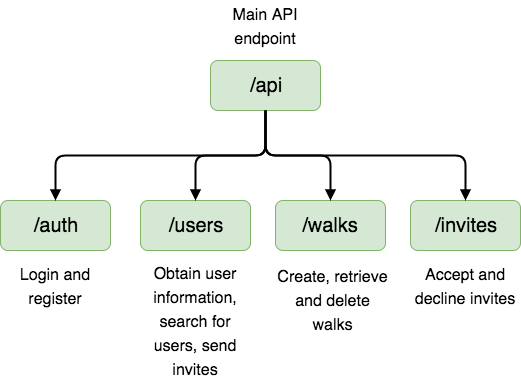
\includegraphics[width=0.7\textwidth]{api-routes}
  \caption{Diagram of each of the routes designed for the API. Each route contains a description of what endpoints exist within that route.}
  \label{fig:api-routes}
\end{figure}

Each endpoint in the API followed the CRUD functions -- standing for Create, Read, Update and Delete. These functions are used to define what operation is being performed when changing data in the database. These functions map to HTTP methods very well, which can then be used in each endpoint to clearly state what operation is used. For example, an endpoint that deletes certain data from the database should adopt the \textit{Delete} function of CRUD and therefore also use the DELETE HTTP method.

\subsection{User Authentication}

For a user to be able to save their tracked walks and invite other users to go on a walk, an authentication system needs to be used. There are two types of authentication that can be used to identify a user when making a request to the API:

\begin{itemize}
  \item \textbf{Basic authentication} requires a username and password, which are compared against the values stored in the database and authenticates the user if these values match.

  \item \textbf{Token-based authentication} authenticates the user through a unique key given to the client by the API, and can restrict access to certain functions of the API depending on that user.
\end{itemize}

Basic authentication alone is the only method necessary for an application to support user authentication and multiple device registration. The best practice however is to use basic authentication along with token-based authentication to prevent passwords having to be re-entered. For example, when just using basic authentication, any restricted API request would require the user to enter their username and password again, which can get extremely tedious. When using token-based authentication, this key can be stored on the client-side when it is first received upon login or registering an account, and can then be used in subsequent API requests without the need for re-authentication.

A way to secure the authentication system even more is to create access tokens using a JSON Web Token (JWT). These are tokens that are digitally signed and encoded, meaning that source of the data can be verified when sending a request from the client to the API. JWT is also implemented in Node.js and can therefore be both verified and signed directly from the API. There are alternatives to using JWT, such as services like OAuth that better deal with user sessions, however the overhead required to set up OAuth would not be worthwhile.

Using both basic and token-based JWT authentication, the authentication system of the API could be designed. When the client sends a request to login using their username and password, basic authentication is used and a JWT is returned by the API if the authentication is successful. The returned JWT is then stored by the client and if any API requests specify that authorisation is required, the JWT is sent in the \textit{Authorization} header of the request.
 
\subsection{File Storage Methods} \label{subsection:file-storage-methods}

There are two methods that can be used when uploading images via an API to a file storage service such as AWS S3. The first of which is direct upload where the client -- the mobile app in this case -- uploads the file directly to S3, bypassing the API altogether. The other option, known as pass-through upload, is to upload the image via a request to the API and then let the API handle the upload to S3. The former of the two options is the most commonly used since it does not require any extra processing to be performed by the API, which could result in slower response times especially on Heroku.

While the direct upload method does also require a slightly more complicated implementation, I decided to choose it based on the needs of this project and its ability to be scaled effectively.

\section{Summary}

The design section outlined the elements of the project that needed to be completed before any implementation could begin. The basic user interface design of the main screens of the mobile application were created using the MVC design pattern, allowing for front-end development to begin. Meanwhile, the structure of the database and endpoints in the API meant that implementation in the back-end could begin by using the technologies chosen in Section \ref{section:technologies}. 





